%!TEX root = main.tex
\section{Experiments}\label{sec:exp}

\subsection{Experimental Setup}
We have used the Frames dataset \cite{frames} as 
our benchmark. Containing 1369 dialogs between 
a chatbot and users interested in booking a vacations, 
it consists the entire dialogs along with its semantic features. 
Each dialog is assigned a tag of 1 if the user has booked a vacation 
in the dialog and 0 otherwise. 61\% of the dialogs end with a user 
booking a vacation and the average length of a dialog was 14 turns. 

Since originally this dataset was not created for the dialog-end problem, 
we had tagged all dialogs automatically, using other features that exist 
in the dataset, namely sentences that include a ``book'' action. 

Starting from the word embeddings, we have used the 
NLTK package \cite{DBLP:conf/acl/Bird06} and the already trained network GloVe \cite{glove} 
to embed the words in each sentence to vectors using the the Keras package \cite{chollet2015}. 
We then use Keras to build our hierarchal network, train it and test it on the 
dataset, with the exception of the attention layers applied on both the word and sentence 
levels, inspired by the concepts presented in \cite{attention}. 
The hyper-parameters in our experiments are as follows. 
Word embedding dimension is set to 100 and the 
LSTM dimension is set to 50. 

We have divided the dataset into 80\% training dialogs and 20\% test dialogs 
(some of the dialogs were too short to be included, containing only 3 or less sentences).
Training was performed with a mini-batch of size 20, 
and 20 epochs.
% Our network used SGD with a momentum of 0.9 \amir{verify} to train.

\subsection{Baselines}% and Results
To our knowledge, no solution for the 
dialog-end problem has been previously proposed. To nevertheless
gain insight on alternatives, we have tested various configurations 
of the network. 
The different configurations of the network include: 
(1) adding the additional turn-level encoding, 
(2) including word and sentence level attention, 
(3) including turn-level attention, and 
(3) varying $k$ (recall Definition \ref{def:target}).

We have examined all configurations that do not use/use options 
(1), (2), and (3) with three different values of $k$, namely $4,8$ and 
the full dialog. For further comparison, we examined the performance of a naive bag-of-words 
approach. 
We have also experimented with different parameters of the network. 
In particular, the dimensionality of the LSTM output was adapted towards 
the best performing configuration.

% \begin{enumerate}
% 	\item Standard bag-of-words implementation using only the text.\label{b:1}
% 	\item Character-level CNN model using only the text \cite{ZhangZL15}.\label{b:2}
% 	\item Bidirectional RNN with LSTM whose input included only the semantic features detailed in Section \ref{sec:semantic}.\label{b:3}
% 	\item The hierarchical attention network for document classification \cite{attention} without the semantic features (again, using only the text), with and without attention.\label{b:4}
% 	\item The hierarchical network for document classification \cite{attention} {\em without} the semantic features, with the additional turn layer, and without attention.\label{b:5}
% 	\item The hierarchical network for document classification \cite{attention} {\em with} the semantic features, with the additional turn layer, and without attention.\label{b:6}
% \end{enumerate}

% The latter two baselines are in fact components 
% of our network so comparing their performance to 
% the network we have designed can lead to insights 
% on the amount of improvement given by combining them. \amir{is there an improvement?}


\subsection{Results}
% To examine the usefulness of our approach and 
% test the effectiveness of the different components, 
% we have evaluated the different baselines on the Frames 
% dataset \cite{frames} and examined the two main components of our network separately 
% and with the values $k=4$, $k=8$, and when the input is the full dialog (recall Definition \ref{def:target}). 

% \begin{table*}[!htb]
%     \centering\small
%     \begin{tabular}{| c | c | c | c | l | l |}
%         \hline \textbf{Solution} & \textbf{$k=4$} & \textbf{$k=8$} & \textbf{Full Dialog} \\
%         \hline Baseline \ref{b:1} & TBD & TBD & TBD \\
%         \hline Baseline \ref{b:2} & TBD & TBD & TBD \\
%         \hline Baseline \ref{b:3} & 62 & 75 & 76 \\
%         \hline Baseline \ref{b:4} without attention  & 65 & 69 & 86 \\
%         \hline Baseline \ref{b:4} with attention  & 65 & 70 & 91 \\
%         \hline Baseline \ref{b:5} & 67 & 72 & 88 \\
%         \hline Baseline \ref{b:6} & 61 & 72 & 88 \\
%         \hline This Project & TBD & TBD & TBD \\
%         \hline
%     \end{tabular}
%     \caption{Precision in Dialog-End Classification}\label{tbl:resComps}
% \end{table*}


\begin{table*}[!htb]
    \centering\small
    \begin{tabular}{| c | c | c | c | c | c |}%{\bf Attention On Words and Sents}
        \hline \textbf{Turn Layer} & \begin{tabular}{@{}c@{}}{\bf Attention On} \\{\bf Words and Sents}\end{tabular} & \textbf{Attention On Turns} & \textbf{k} & \textbf{Accuracy} \\
        \hline No & No & No & 4 & 67.7 \\
        \hline No & Yes & No & 4 & 66.9 \\
        \hline Yes & No & No & 4 & 69.2 \\
        \hline Yes & Yes & No & 4 & 66.1 \\
        \hline Yes & Yes & Yes & 4 & 62.2 \\
        \hline Yes & No & Yes & 4 & TBD \\
        \hline No & No & No & 8 & 69.8 \\
        \hline No & Yes & No & 8 & 73.4 \\
        \hline Yes & No & No & 8 & TBD \\
        \hline Yes & Yes & No & 8 & 57.2 \\
        \hline Yes & Yes & Yes & 8 & 67.1 \\
        \hline Yes & No & Yes & 8 & TBD \\
        \hline No & No & No & full dialog & 84.6 \\
        \hline No & Yes & No & full dialog & 84.9 \\
        \hline Yes & No & No & full dialog & 89 \\
        \hline Yes & Yes & No & full dialog & 92.3 \\
        \hline Yes & Yes & Yes & full dialog & 89.3 \\
        \hline Yes & No & Yes & full dialog & 93 \\
        
        \hline
    \end{tabular}
    \caption{Accuracy in Dialog-End Classification}\label{tbl:resComps}
\end{table*}


\begin{figure}[]
    \hspace*{-0.8cm}
    \centering
    % \begin{subfigure}[b]{0.55\columnwidth}
        \centering
        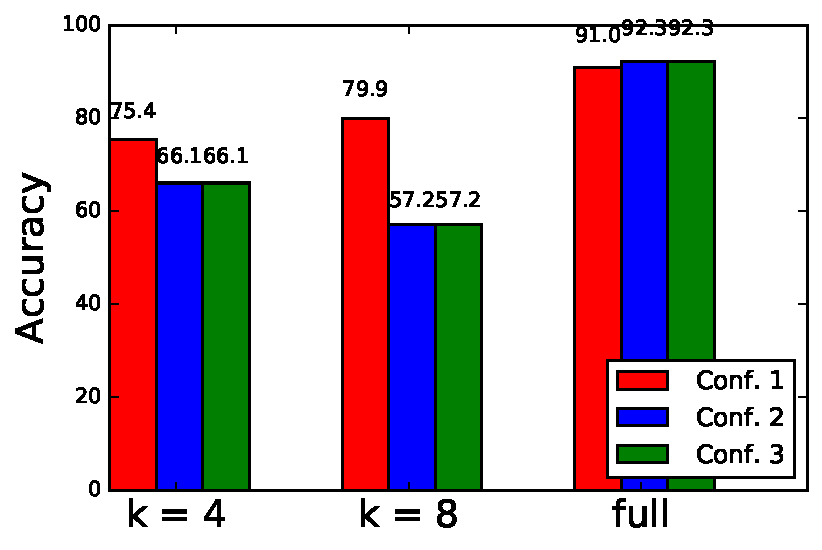
\includegraphics[trim=0cm 0.5cm 0cm 0cm, width=2.5in]{exp/configs.pdf}
        \caption{Performance of Selected Configurations}
        \label{graph:quality}
    % \end{subfigure}%
    % \begin{subfigure}[b]{0.45\columnwidth}
    %     \centering
    %     \includegraphics[trim=0cm 0.5cm 0cm 0cm, width=1.6in]{experiments/sp2b_quality_k.pdf}
    %     \caption{Increasing $k$}
    %     \label{graph:qualityK}
    % \end{subfigure}
    % \caption{Percentage of Success for SP2B}
    % \label{fig:quality}
    % \vspace{-4mm}
\end{figure}


The results for the different structures of the network are shown in Table \ref{tbl:resComps}. 
First, note that our novel configuration with the turn layer and attention on the turns alone 
performs better than the all other configurations (specifically, the one given in \cite{attention}) 
reaching \amir{complete} for $k=8$ and 93\% accuracy for the full dialog. 
All configurations show an improvement in performance with the increase of $k$, 
except a single one which we will explain in the sequel. 
Configurations that include a turn layer with the attention mechanism applied on all layers 
tend to overfit the data reaching up to 99\% accuracy during training but 
dropping up to 57.2\% accuracy during testing. 
This suggests that these configurations are too complex for the amount of data in our dataset. 
Further note that for smaller values of $k$, the attention mechanism 
(for words and sentences, turns, and both) damages performance due to overfitting. 
However, for the full dialog, there is an improvement of up to 4\%. 
This stems from the mechanism's need for a larger volume of text.

Figure \ref{graph:quality} shows a comparison between three of the configuration 
we have examined, where Config. 1 is a standard implementation of bag-of-words, 
Config. 2 is the network shown in \cite{attention}, and Config. 3 is the configuration 
we present in this project, namely \amir{take best config}. 
All three networks perform well based in all three cases. 
We can see that for $k=4,8$, bag-of-words outperforms the more complex 
networks \amir{decide if }

% Since the hierarchical network without the turn-layer is focused on the text itself, 
% it is much more affected by the addition of new text than other structures, where more semantic features 
% do not necessarily imply novel information \amir{make sure}. 
% Thus, the semantic features based approach (baseline \ref{b:3}) is considerably 
% less sensitive to an increase in $k$ than the hierarchical network. 
% Further note that for smaller values of $k$, the attention mechanism 
% does not increase performance by a major factor (1\% at most). This again stems from 
% the mechanism's need for a larger volume of text. As evidence, there is 
% an improvement of 5\% over the full dialogs. 
% We can see that adding the additional layer for turns assists the network in the 
% classification from the comparison between baselines \ref{b:4} and \ref{b:5} for $k=4,8$. 
Interestingly, the semantic features do not seem to improve the performance 
when they are add to the turn vector.


% \paragraph*{Baselines \ref{b:1}, \ref{b:2}}





% \paragraph*{Baselines \ref{b:3}, \ref{b:4}}
% The results for baselines \ref{b:3}, \ref{b:4}, \ref{b:5}, \ref{b:6} are shown in Table \ref{tbl:resComps}. 
% All baselines show an improvement in performance with the increase of $k$. 
% Since the hierarchical network analyzes the contexts and models the text itself, 
% it is much more affected by the addition of new text than the semantic RNN (baseline \ref{b:3}) where more semantic features 
% do not necessarily imply novel information. 
% Thus, the semantic features based approach (baseline \ref{b:3}) is considerably 
% less sensitive to an increase in $k$ than the hierarchical network. 
% Further note that for smaller values of $k$, the attention mechanism 
% does not increase performance by a major factor (1\% at most). This again stems from 
% the mechanism's need for a larger volume of text. As evidence, there is 
% an improvement of 5\% over the full dialogs. 
% We can see that adding the additional layer for turns assists the network in the 
% classification from the comparison between baselines \ref{b:4} and \ref{b:5} for $k=4,8$. 
% Interestingly, the semantic features do not seem to improve the performance 
% when they are add to the turn vector.
